%%%% ijcai11.tex

\typeout{IJCAI-11 Instructions for Authors}

% These are the instructions for authors for IJCAI-11.
% They are the same as the ones for IJCAI-07 with superficical wording
%   changes only.

\documentclass{article}
% The file ijcai11.sty is the style file for IJCAI-11 (same as ijcai07.sty).
\usepackage{ijcai11}
\usepackage{mathtools}
\usepackage[utf8]{inputenc}

% For importing images.
\usepackage{graphicx}

% The language we want and appropriate hyphenation.
\usepackage[dutch]{babel}

% Hyphenation rules.
\hyphenation{biopotentiaal-schommelingen}

% Use the postscript times font!
\usepackage{times}

% the following package is optional:
%\usepackage{latexsym} 


\title{TODO Titel}
\author{Kevin Boets \\ Katholieke Universiteit Leuven\\ Leuven, Belgium \\ kevin.boets@student.kuleuven.be
\And
Gertjan Franken \\ Katholieke Universiteit Leuven\\ Leuven, Belgium \\ gertjan.franken@student.kuleuven.be}

\begin{document}

\maketitle

\begin{abstract}
In de zoektocht naar natuurlijke user interfaces gebeurt er onderzoek naar besturing door middel van de ogen. In deze paper wordt gebruikgemaakt van EMG (Elektromyografie) signalen om eenvoudige oogbewegingen te detecteren. Hiervoor geeft men twee verschillende methodes: thresholds en patronen. Beide methodes worden dan ook grondig besproken en vergeleken doorheen de tekst.
\end{abstract}

\section{Introductie}

Reeds verschillende manieren om oogbewegingen te detecteren zijn bedacht. Zo kan men al door middel van camera's de ogen volgen. Hierbij gaat men op zoek naar de positie van de iris om de stand van het oog te achterhalen. Deze technieken zijn al ver ontwikkeld, maar toch gaan we nu een andere techniek onderzoeken. Aan de hand van de EMG signalen die gemeten worden door middel van sensoren die rond de ogen zijn aangebracht, proberen we te achterhalen in welke richting de gebruiker kijkt. Als invoer krijgen we twee elektrooculogrammen die de de kijkrichtingen links-rechts en boven-onder voorstellen. Figuur ~\ref{fig:originaldata} geeft een mooi voorbeeld weer van het elektrooculogram betreffende de kijkrichtingen links en rechts. Hierbij stellen de dalen de kijkrichting links voor en stellen de bergen de kijkrichting rechts voor.

\section{Preprocessing}

De signalen die we krijgen doorgestuurd, afkomstig van de sensoren, zijn zeer ruw. Om hier kijkrichtingen uit af te kunnen leiden, gaan we de data eerst beter leesbaar maken. Dit is de preprocessing-stap. Deze stap voeren we uit op elke dataset,  alvorens we deze gaan analyseren. Beschouw de data in figuur ~\ref{fig:originaldata} als de originele data.

\begin{figure}[h]
\centering
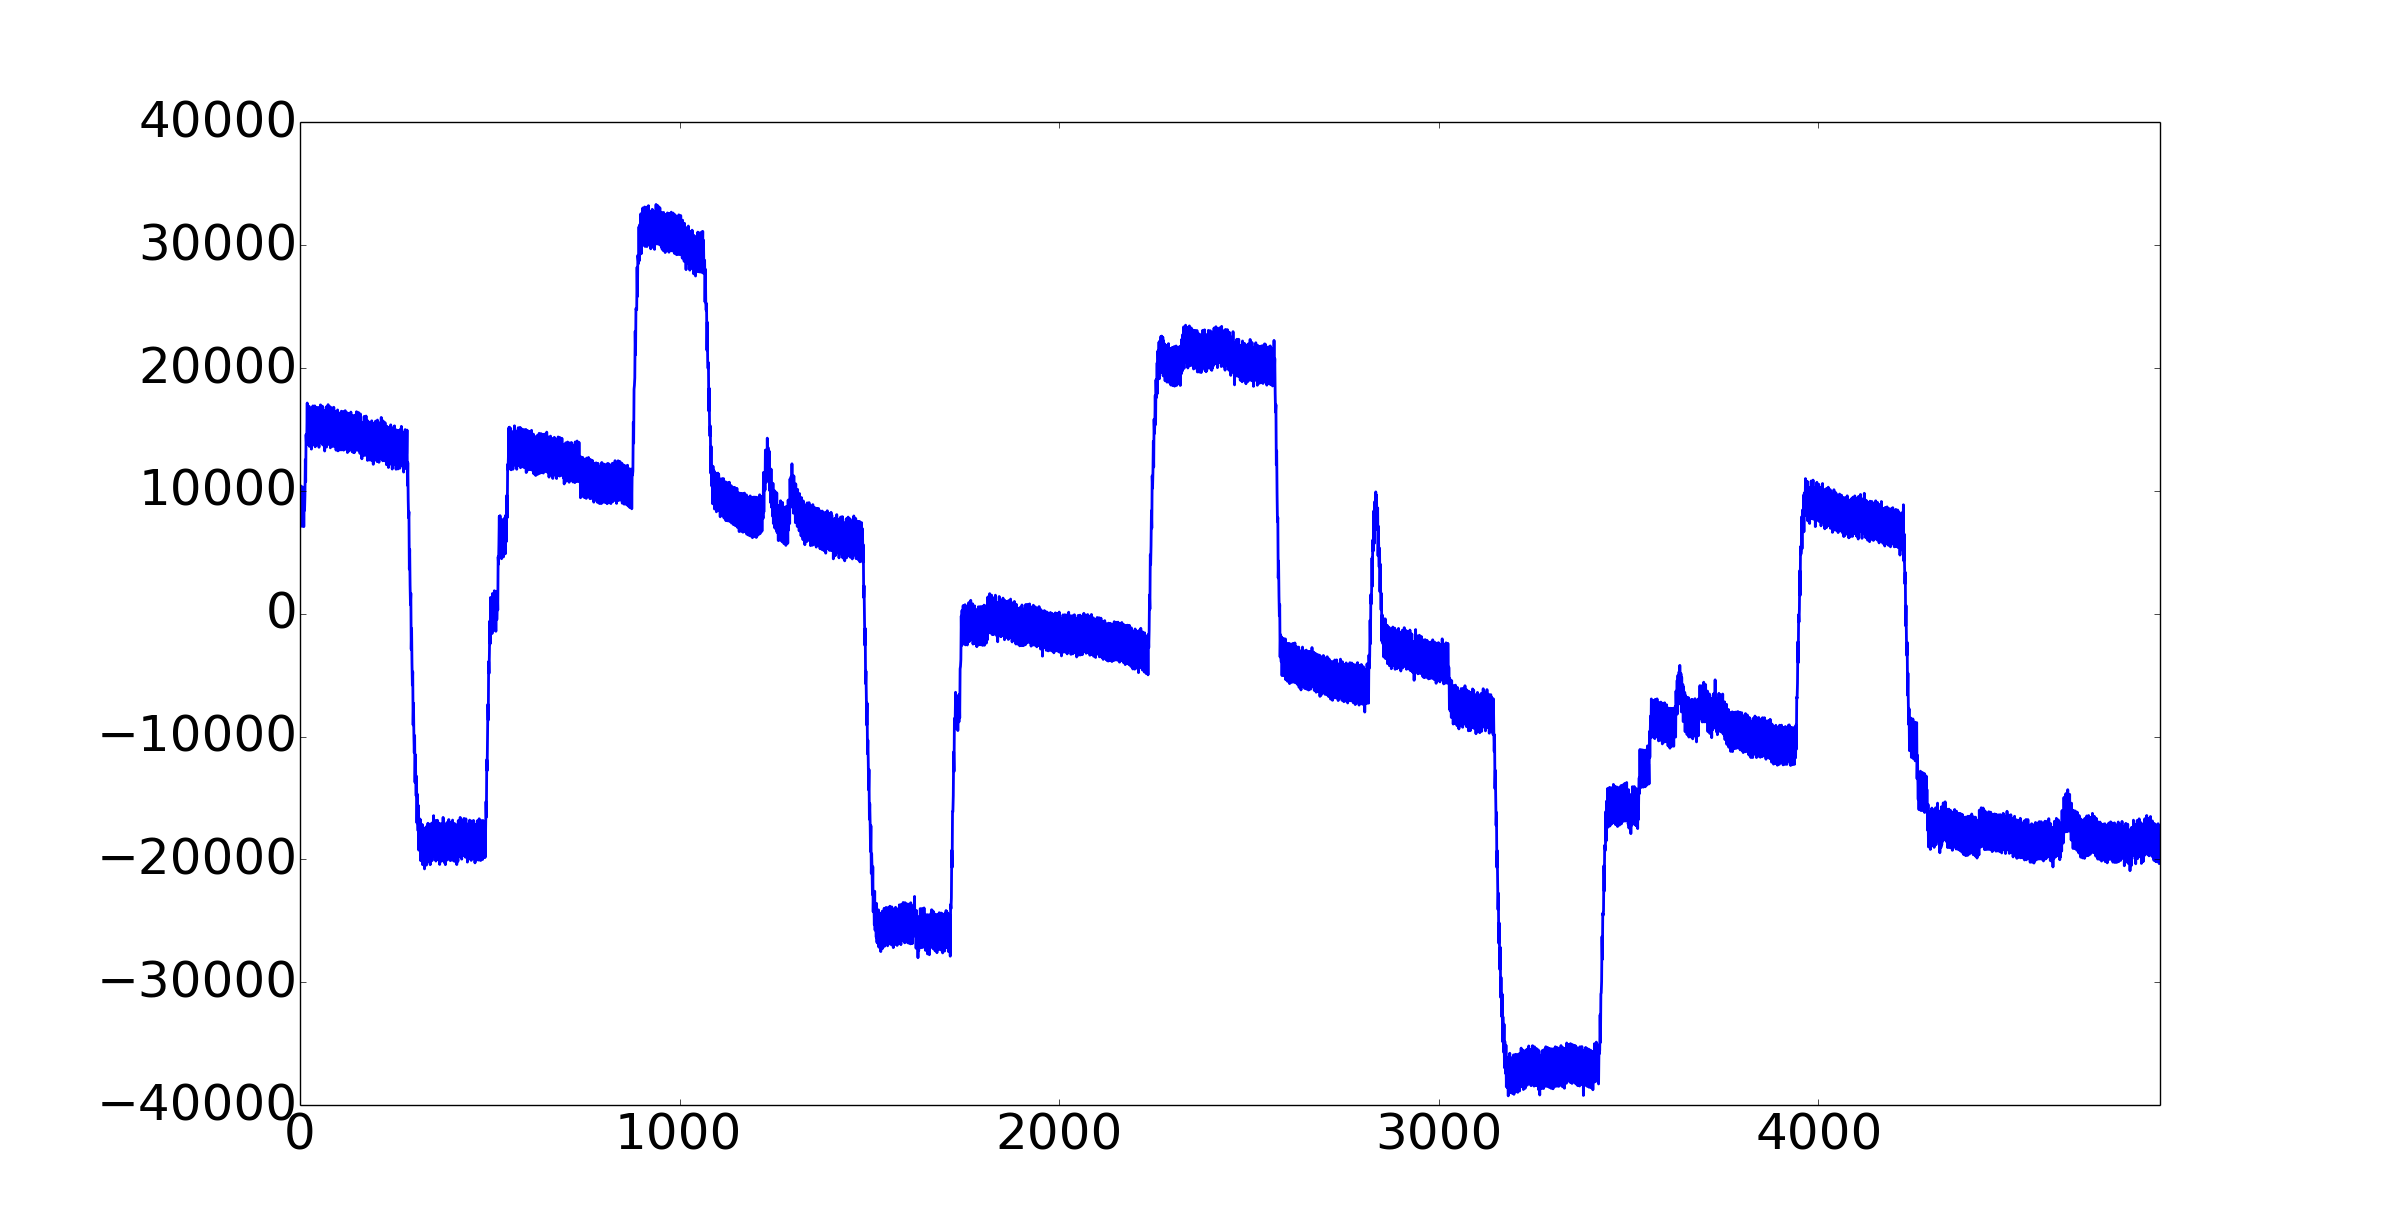
\includegraphics[width=\linewidth]{images/original_data}
\caption{Originele data rechtstreeks afkomstige van de hardware. De grootheid op de x-as is tijd en op de y-as is dit het voltage.}
\label{fig:originaldata}
\end{figure}

Als eerste gaan we de ruis en knipperingen zo goed mogelijk proberen te verminderen. Dit gebeurt door middel van een low-pass filter. Deze filter verzacht alle signalen waarvan de frequentie hoger is dan onze cutoff frequentie. [TODO berekenen wat onze cutoff frequentie is].

Daarna focussen we ons op de biopotentiaalschommelingen. Deze schommelingen kunnen we niet op voorhand voorspellen en verschillen van persoon tot persoon. Als we deze schommelingen kunnen verminderen, kunnen we meer steunen op absolute waardes van het signaal. In dit tweede deel van de preprocessing-stap gebruiken we opnieuw een low-pass filter. Deze keer gebruiken we een lage cutoff frequentie [TODO weer cutoff berekenen]. Na deze filtering van de data, blijven enkel de signalen met een lage frequentie over. Het resultaat is de benadering van de biopotentiaal van de gebruiker die doorheen de tijd fluctueert. We kunnen nu de biopotentiaalschommelingen uit onze originele data verminderen door de gevonden benadering hiervan af te trekken. De schommelingen verdwijnen niet volledig, maar worden wel sterk verminderd. Figuur ~\ref{fig:filtereddata} stelt het resultaat van de besproken filtereringen voor.

Bij veelvuldige herhaling van dezelfde kijkrichting, wordt een probleem in verband met deze methode zichtbaar. Als er veel en opeenvolgend naar éénzelfde richting gekeken wordt, zullen de waarden in de data algemeen lager of hoger zijn. De gefilterde data zal hierdoor ook algemeen lager of hoger liggen. Dit is een probleem aangezien het de benadering van de biopotentiaal moet voorstellen. Doordat de gevonden benadering foutief is, zullen ook alle volgende bewerkingen een incorrecte uitkomst hebben. Wanneer we dus deze benadering aftrekken van de oorspronkelijke data, zal de data ongewenst verschuiven volgens de y-as. Hierdoor zal het werkend met absolute waarden slechte resultaten leveren. Om dit te verkomen, zullen we er voor zorgen dat er wordt gewisseld van kijkrichting, waar mogelijk.

\begin{figure}[h]
\centering
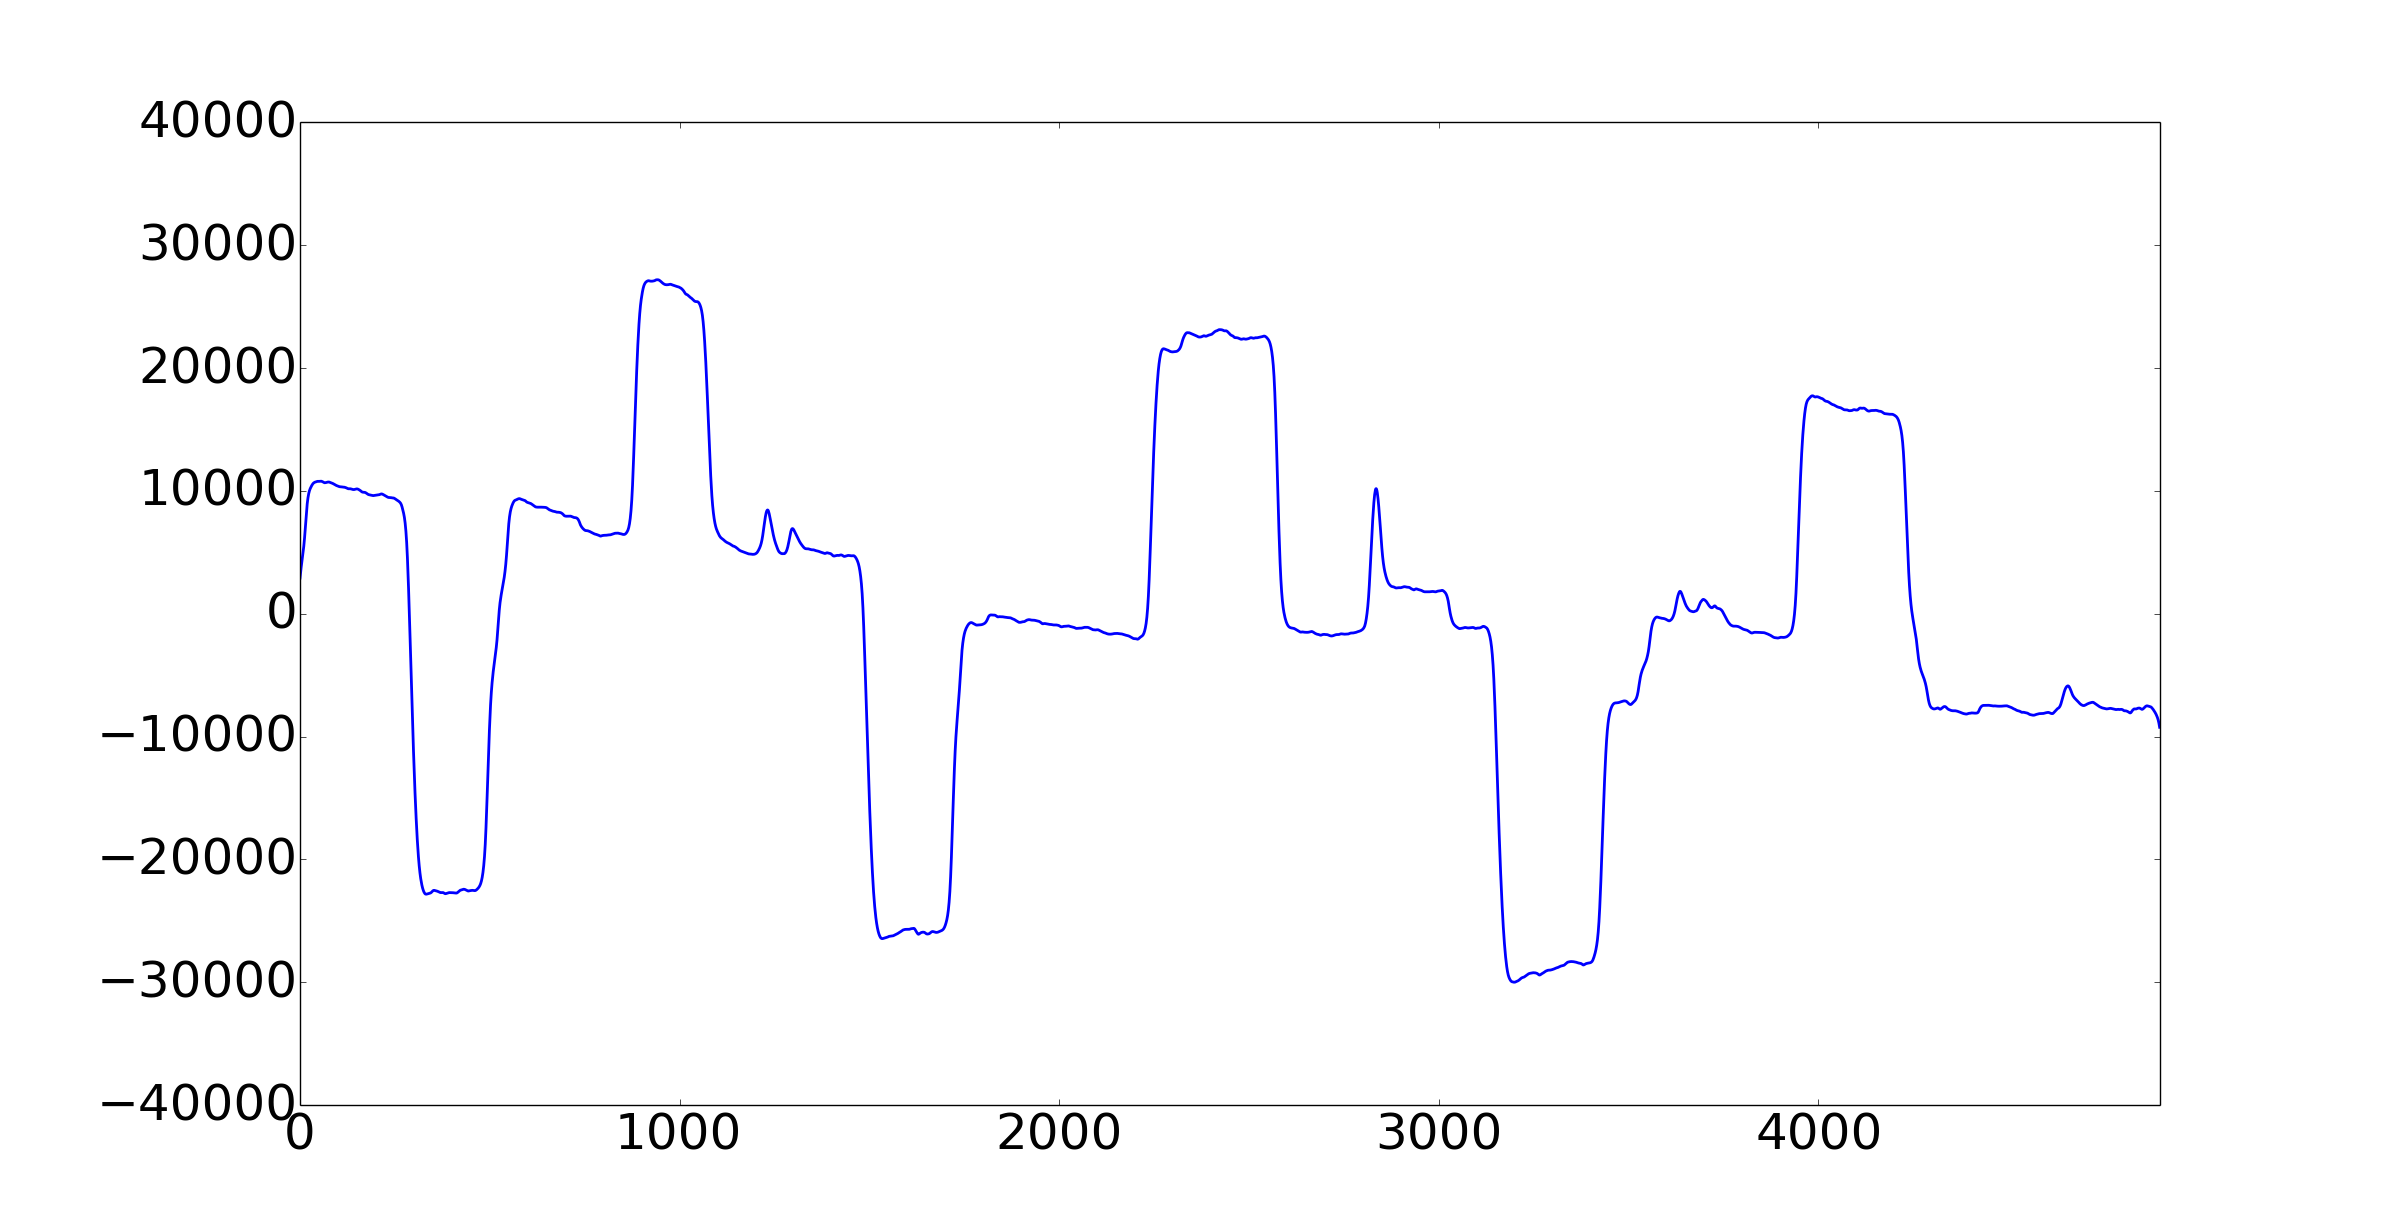
\includegraphics[width=\linewidth]{images/filtered_data}
\caption{Het resultaat van de twee filteringen op de originele data. De ruis is sterk verminderd en de sterkte van de knipperingen is afgenomen. De biopotentiaalschommeling is niet helemaal weg, maar wel voldoende verminderd.}
\label{fig:filtereddata}
\end{figure}

Na toepassing van de vorige filteringen, discretiseren we de data. Deze stap is eerder optioneel en wordt enkel in de methode met patronen gebruikt. Het grote voordeel van deze stap is dat we minder berekeningen zullen moeten doen, wat de uitvoeringstijd van het programma ten goede komt. Hiervoor gebruiken we de SAX-discretisatie (Symbolic Aggregate approXimation) \cite{sax}. De verdeling van de letters die het SAX-woord opmaken, bepalen we op de volgende manier. Om een goede verdeling te hebben, moeten de letters ongeveer even veel voorkomen. Eerst wordt de data genormaliseerd. We definiëren op voorhand hoeveel waarden een letter voor moet stellen. Dit is de constante $w$. De data die we willen discretiseren, verdelen we op in partities van lengte $w$. Elke partitie zal een bepaalde letter krijgen, afhankelijk van zijn gemiddelde. Het aantal verschillende letters dat we gebruiken, hangt af van de alfabetgrootte $a$. Volgens de normale verdeling wordt nu elke partitie aan een letter gekoppeld. Zie Figuur ~\ref{fig:discretization} voor de visuele werking. Eigenlijk stelt elke letter nu een reeks van waarden voor. Om SAX-woorden voor te kunnen stellen in grafieken, geven we elke letter ook een waarde. Dit is het gemiddelde van het interval dat de letter op zicht neemt.

\begin{figure}[h]
\centering
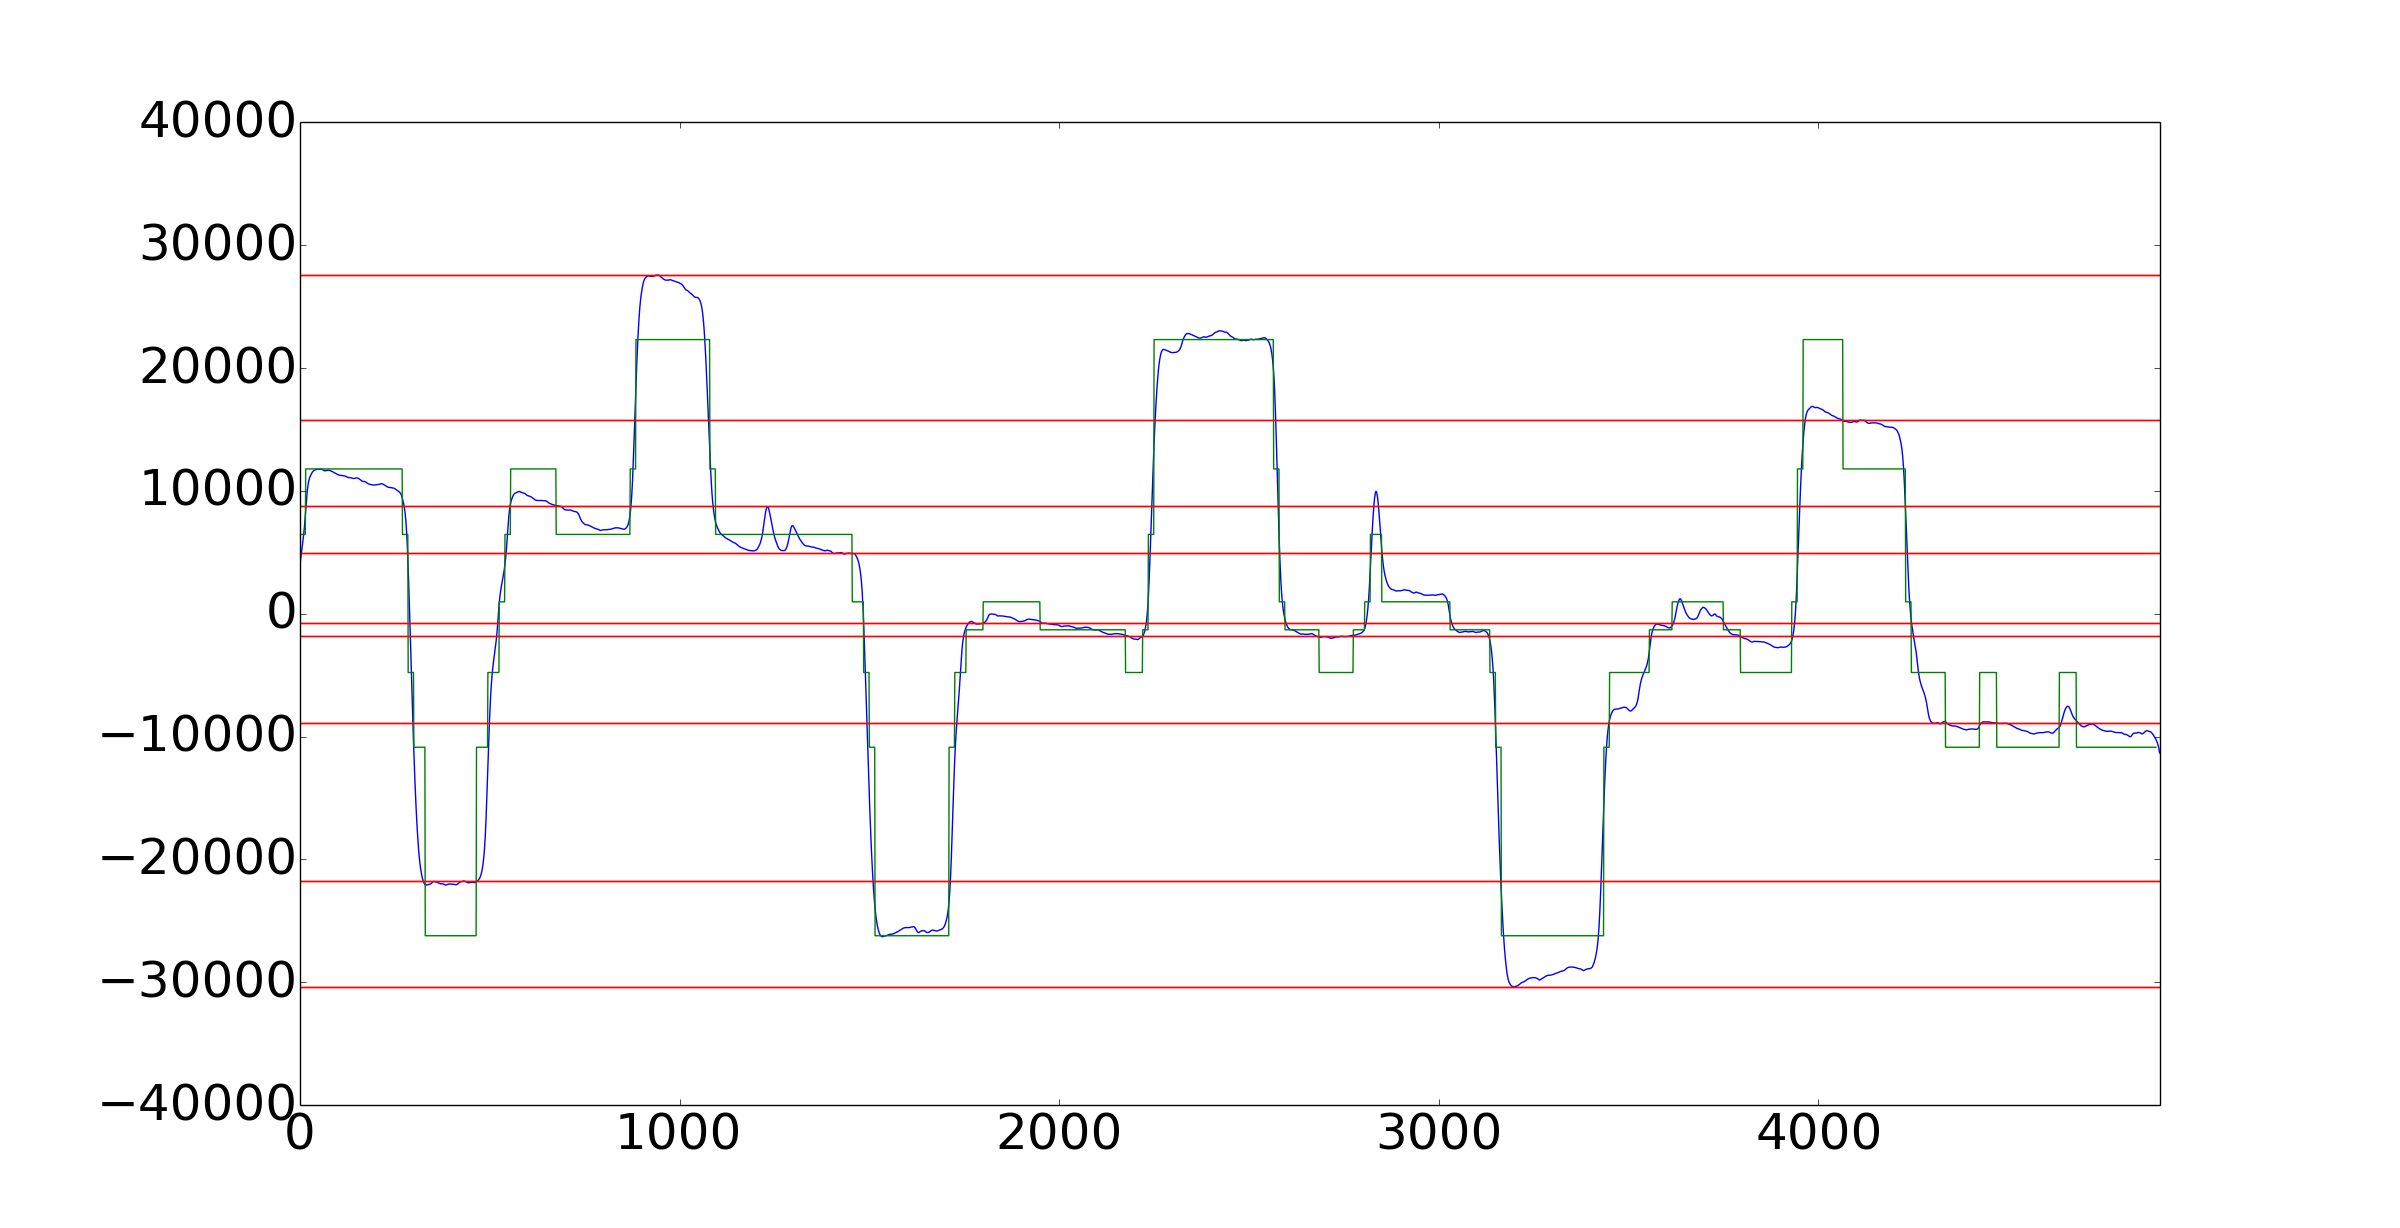
\includegraphics[width=\linewidth]{images/discretized_data}
\caption{De groene lijn stelt de discretisatie voor van de gefilterde data die in het blauw staat. De rode horizontale lijnen geven de distributie weer van de SAX-letters.}
\label{fig:discretization}
\end{figure}

[TODO andere afbeelding van discretisatie]

\section{Gebruikte methoden}

In ons onderzoek hebben we gebruik gemaakt van twee verschillende methoden om kijkrichtingen te herkennen. Deze methoden steunen respectievelijk op thresholds en patronen. Beide methoden beginnen met een calibratie-fase, gevolgd door een herkennings-fase. In de calibratie-fase laten we de gebruiker naar een aantal richtingen kijken, waarna we deze data analyseren. De gevonden informatie koppelen we aan de juiste kijkrichting. In de herkennings-fase wordt deze informatie gebruikt om in de nieuwe data kijkrichtingen te detecteren.

\subsection{Thresholds}

De eenvoudigste methode is de methode gebruikmakend van thresholds. Hij steunt vooral op de absolute waarden van de data. Het basis idee van deze methode is als volgt. Er wordt een bovengrens gedefinieerd voor elke kijkrichting in de calibratie-fase. Als deze overschreden wordt in de herkennings-fase, gaan we er van uit dat er in de overeenkomstige kijkrichting gekeken wordt.

In de calibratie-fase wordt aan de gebruiker gevraagd om een bepaalde sequentie van kijkrichtingen uit te voeren. Vervolgens voeren we de preprocessing in verband met de ruis, knipperingen en biopotentaail uit. De verschoonde dataset gebruiken we dan om goede bovengrenzen te vinden.


\begin{figure}[h]
\centering
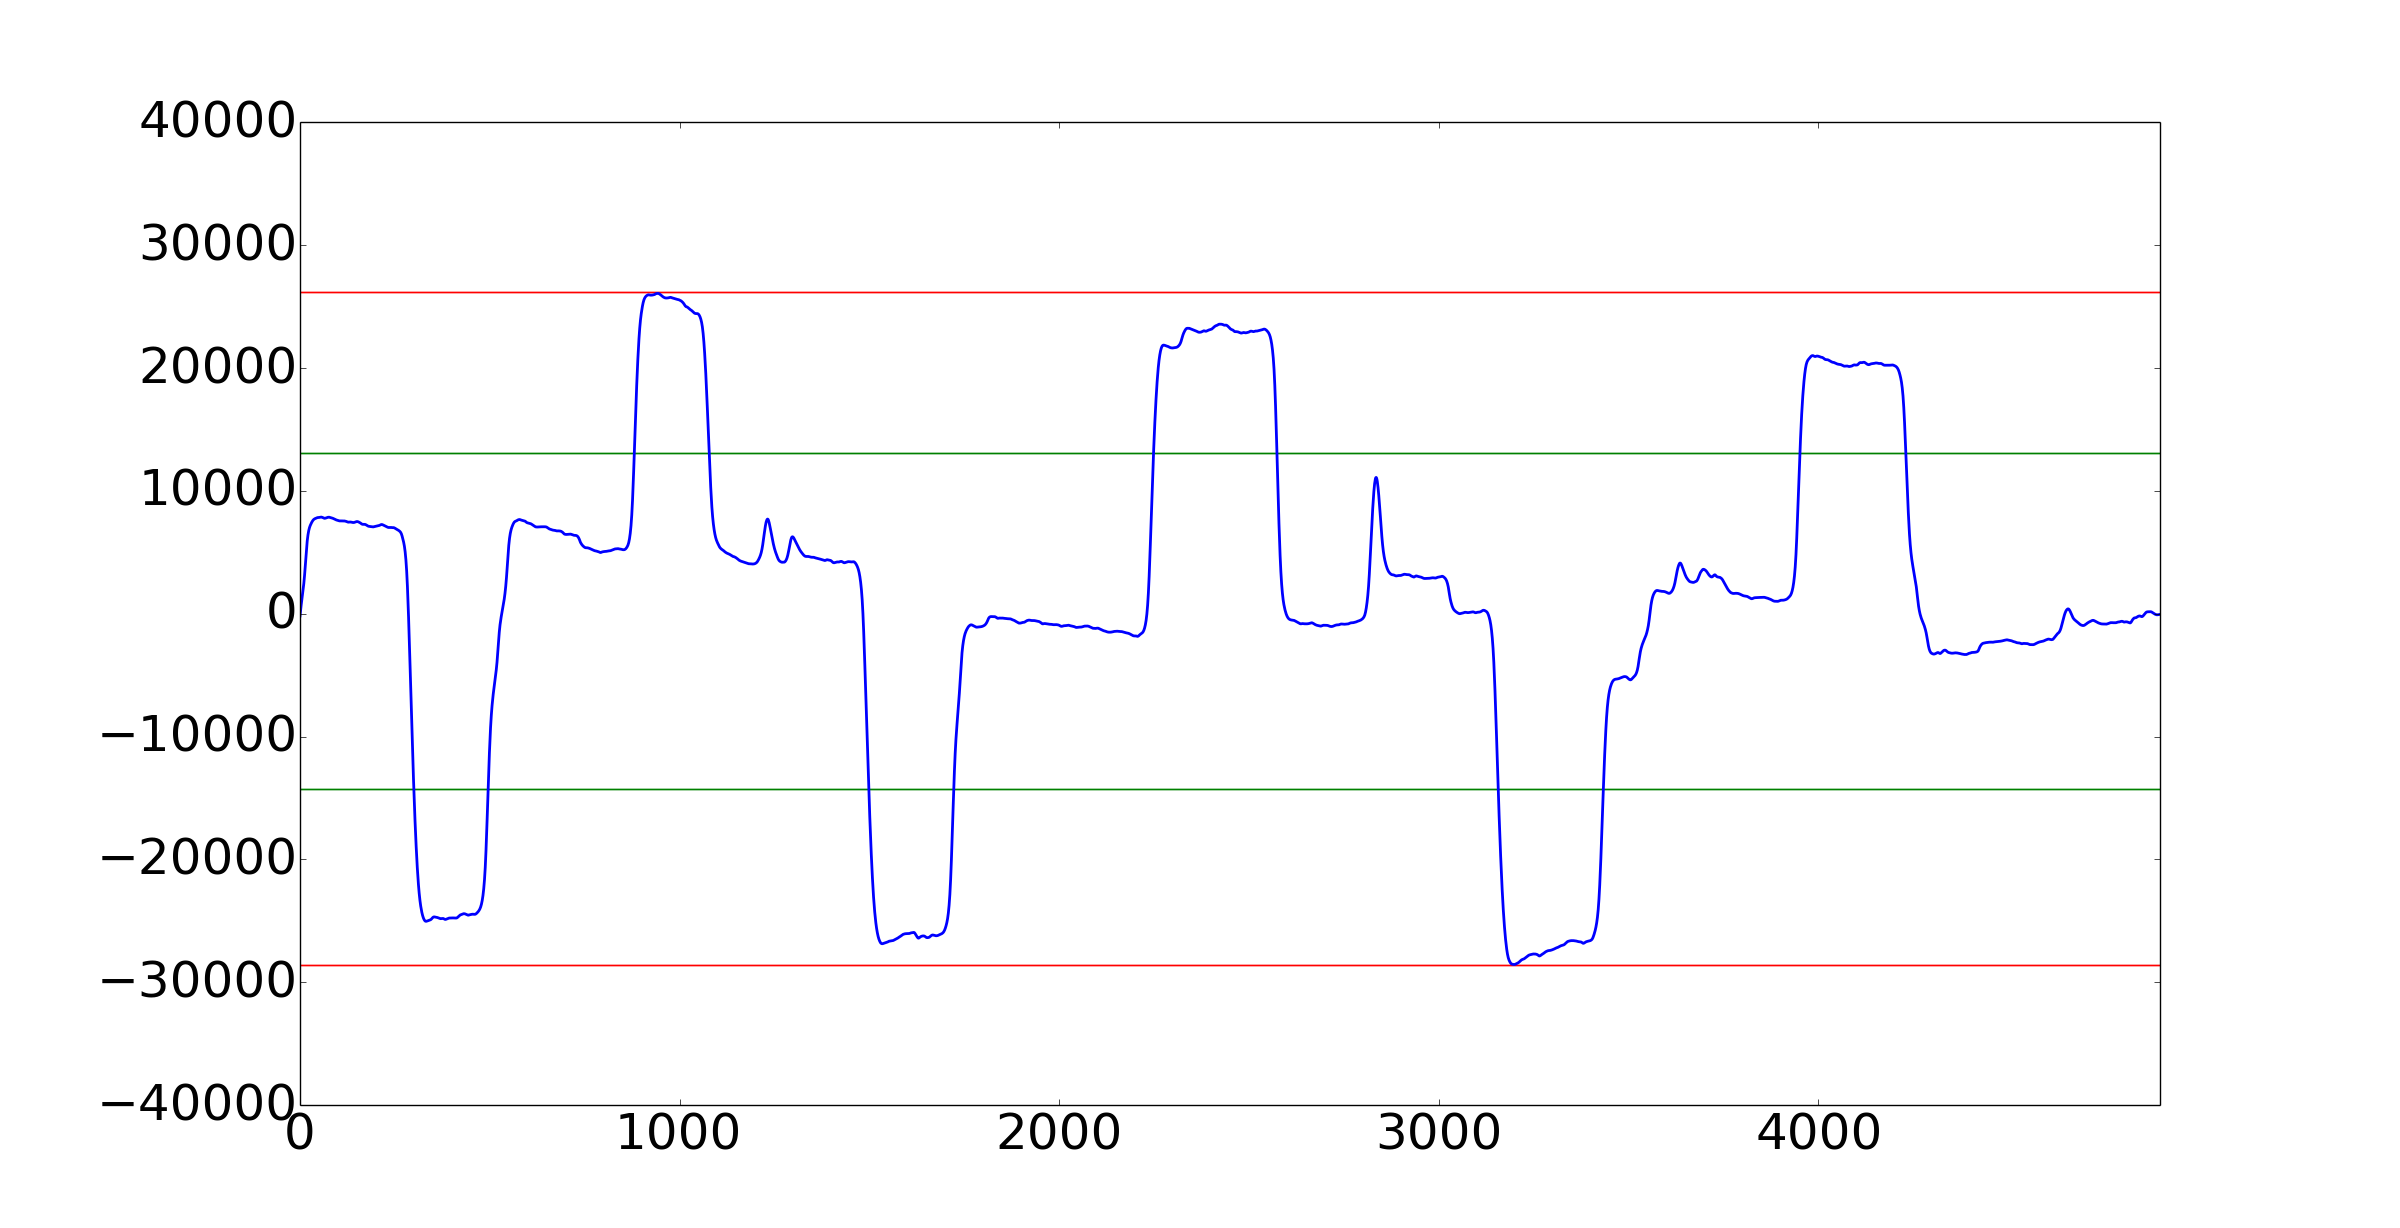
\includegraphics[width=\linewidth]{images/thresholds_distribution}
\caption{In deze afbeelding stellen de rode lijnen het minimum en maximum voor. De groene lijnen zijn het minimum en maximum vermenigvuldigd met $\alpha$.}
\end{figure}

[TODO andere afbeelding]

[TODO meer zeggen over de nieuwe data?]
Eens we de bovengrenzen hebben gevonden, kunnen we deze in de herkennings-fase gebruiken om kijkrichtingen detecteren. Om deze gevonden bovengrenzen te kunnen gebruiken, zullen we eerst dezelfde preprocessing stappen utivoeren op de nieuwe data.

[TODO 'overschreden  duidelijk genoeg?]
Om kijkrichtingen te detecteren, gaan we de bovengrenzen vergelijken met de waardes uit de data. Wanneer een bovengrens overschreden wordt, toont dit aan dat de gebruiker mogelijk in een van de richtingen aan het kijken is. Dit kunnen we echter niet zomaar aannemen. Een enkele piek, zoals een knippering, zou dan ook ongewild worden herkend als kijkrichting. Om voor meer zekerheid te zorgen, wachten we tot dezelfde grens opeenvolgend meerdere keren overschreden is. Hoeveel keren definiëren we op voorhand. Het aantal dat we kiezen is een afweging tussen detectiekans en zekerheid. Bij een klein aantal is de kans op detectie hoog, maar zijn we minder zeker over de geldigheid van de detectie. Een groot aantal zal anderzijds veel zekerheid verschaffen, waarbij er wel een grotere kans is dat korte kijkrichtingen niet worden gedetecteerd. Hierbij is een goede balans belangrijk.

\subsection{Patronen}

In tegenstelling tot de thresholds-methode, steunt deze methode weinig op absolute waarden en eerder op relatieve waarden. Er wordt naar motieven gezocht in de calibratie-fase, die dan in de herkennings-fase met de nieuwe data vergeleken worden \cite{motifs}. In deze methode maken we gebruik van SAX-woorden om de efficiëntie te verhogen.

Ook hier wordt in de calibratie-fase aan de gebruiker gevraagd om in een aantal kijkrichtingen te kijken. Voor elke kijkrichting hebben we nu een aantal datasets van signalen die we met elkaar gaan vergelijken. Voor elke kijkrichting zoeken we de meest succesvolle motieven. Dit zijn de motieven die het meest aantal matches hebben. We zeggen dat twee sequenties met elkaar matchen indien deze voldoende hard op elkaar lijken. Hiervoor moeten specifieke voorwaarden gedefinieerd worden, dit doen we voor ons programma in de implementatie-sectie.



De gevonden motieven, gekoppeld aan de bijhorende kijkrichtingen, worden doorgegeven aan de herkennings-fase. De binnenkomende data wordt verdeeld in sequenties die omgezet worden in SAX-woorden. Pas als er een match is tussen een binnengekomen SAX-woord en een SAX-woord van een motief, vergelijken we deze sequenties op preciezer niveau. Als deze sequenties weer goed genoeg op elkaar lijken, gaan we uit van de kijkrichting gekoppeld aan het motief.

TODO

\section{Implementatie}

Bij het implementeren van ons programma, hebben we ons gebaseerd op de twee eerder uitgelegde methoden. In deze sectie leggen we uit hoe we bepaalde problemen hebben kunnen oplossen. [TODO]

\subsection{Thresholds}

TODO

In de calibratie-fase gaan we dus opzoek naar goede bovengrenzen. Na de preprocessing van de dataset, halen we er de kleinste en grootste waarde uit. Deze twee waarden horen elk bij een andere kijkrichting. Per kijkrichting hebben we ook een constante $\alpha$ waarvoor geldt: $0 < \alpha \leq 1$. We vermenigvuldigen $\alpha$ met zijn respectievelijke waarde en beschouwen de uitkomst als de uiteindelijke bovengrens voor de kijkrichting. In ons programma hebben we $\alpha$ voor beide kijkrichtingen de waarde $0.5$ gegeven, maar deze kan veranderd worden naar behoefte. Zo kunnen we de methode bijvoorbeeld strenger maken door $\alpha$ te verhogen. [TODO vemelden welke $\alpha$ wij gebruiken][TODO welke behoefte?]

[TODO uitleg datawindow, maar 1 keer doen.]
Nu we de bovengrenzen hebben gevonden, moeten we kijkrichtingen gaan zoeken in de nieuwe data. Aangezien we niet weten hoe lang deze zal zijn, gaan we maar een beperkt aantal waardes tegelijkertijd beschouwen. Daarom gaan we een soort venster van 1000 waardes bijhouden. Dit venster zullen we over de data laten glijden zodat er steeds 1000 opeenvolgende waarden van de data zichtbaar zijn. Telkens de window verschuift zullen we de preprocessing uitvoeren over de zichtbare waarden. Aangezien enkel de zichtbaar geworden waarden nieuwe informatie bevatten, zullen telkens enkel deze waarden bekijken. Om de invloed van een enkele uitschieter in de data te beperken, nemen we telkens het gemiddelde van de tien nieuwste punten. Dit gemiddelde gaan we dan vergelijken met alle bovengrenzen. Slechts wanneer de grenzen meerdere keren opeenvolgend overschreden worden, zullen we beslissen dat er een kijkrichting is gevonden.

[TODO deeltje beter bij preprocessing? of toch niet? -> zo goed??]
Sinds we telkens opnieuw onze preprocessing gaan doen, moeten oppassen voor het probleem bij veelvulidige herhaling van dezelfde kijkrichting. Aangezien we in de herkennings-fase weinig invloed hebben [TODO hebben/ willen hebben??] over de volgorde van kijkrichtingen, zullen we dit probleem moeten oplossen. We merken dat het probleem zich enkel voordoet wanneer in het venster meerdere kijkrichtingen te vinden zijn. Daarom gaan we er voor zorgen dat dit niet kan voorkomen door het signaal af te vlakken. Telkens er een threshold overschreden wordt, gaan we het gemiddelde van de vorige datapunten berekenen. Vervolgens vervangen we de originele grensoverschrijdende waardes door dit gemiddelde. Hierdoor zal het venster nooit kijkrichtingen bevatten en bijgevolg zal de preprocessing goed verlopen. Het nadeel van deze techniek is dat de data destructief[TODO iets beter dan destructief? onomkeerbaar?] wordt aangepast en zo mogelijk data verloren gaat. Dit heeft echter geen invloed voor dit systeem, aangezien we enkel ge"interesseerd zijn in de nieuwste data.


\subsection{Patronen}

[TODO data window fill]
[TODO groepen]
In de calibratie-fase beschikken we over verschillende datasets die gelinkt zijn aan een bepaalde kijkrichting. Voor elke kijkrichting zoeken we minstens één paar van motieven. Deze motieven noemen we het beginmotief en het eindmotief. Deze motieven nemen elk een deel van de hele kijkrichting voor hun rekening. Om telkens zo een paar te verkrijgen, leggen we een aantal voorwaarden op. Zo mogen de motieven elkaar nooit overlappen en moet elk hiervan een verschil in hoogte bestrijken. Dit laatste zorgt ervoor dat we nooit quasi horizontale lijnen, die weinig informatie bevatten, als motief zullen vinden. Wij hebben hiervoor een minimaal verschil van 5000 datapunten gekozen.

Voordat we de echte sequenties met elkaar gaan vergelijken, doen we dit eerste met hun genormaliseerde SAX-woorden. Zo kunnen we, zonder al te veel berekeningen, achterhalen welke sequenties in aanmerking komen voor een match. Hiervoor gebruiken we maskers die we op een bepaalde manier genereren [TODO welke manier]. Zo een masker dekt telkens enkele letters van twee te vergelijken SAX-woorden af. Voor elk masker houden we ook een collision matrix bij. Die gebruiken we op de volgende manier. Indien alle overgebleven letters van de SAX-woorden overeen komen, dan wordt de overeenkomstige cel in de collision matrix geincrementeerd. Als we voor alle maskers de collision matrix hebben gemaakt, tellen we al deze matrices met elkaar op. Elk paar van SAX-woorden waarvan de waarde in de overeenkomstige cel van de resulterende matrix groter of gelijk is aan de collision threshold, komt nu in aanmerking voor een match. Deze collision threshold hebben we de waarde 7 gegeven. De oorspronkelijke sequenties van de in aanmerking gekomen SAX-woorden worden nu pas vergeleken. Dit doen we door de euclidische afstand tussen deze genormaliseerde sequenties te berekenen. Pas als deze afstand kleiner is dan de vooraf gedefinieerde range, spreken we van een match.

\begin{table}
\caption{Dit is een voorbeeld van een collision matrix. De letters A tot en met D stellen de verschillende SAX-woorden voor. In dit geval hebben SAX-woorden C en D de meeste collisions, namelijk 10, voor het masker van deze collision matrix.}
\centering
\begin{tabular}{ l || c | c | c | c }
& A & B & C & D \\ \hline
\hline
A & / & 4 & 2 & 2 \\ \hline
B & / & / & 6 & 3 \\ \hline
C & / & / & / & 10\\ \hline
D & / & / & / & / \\
\hline
\end{tabular}\par
\end{table}

Tijdens de calibratie, vergroten we de collision matrix dynamisch. Dit doen we zodat na de calibratie-fase, niet alle data in één keer verwerkt moet worden, maar wel al tussen door kan gebeuren. Bij de eerste twee sequenties die worden toegevoegd, wordt nog gewoon een collision matrix opgesteld. Bij de derde en volgende sequenties, wordt er een nieuwe rij en kolom toegevoegd die overeenkomt met de nieuwe sequentie. Hiervoor worden de benodigde cellen berekend en ingevuld.

Nu we per sequentie het aantal matches hebben, kunnen we een rangschikking maken. We sorteren alle sequenties op het aantal matches dat ze hebben, met de sequentie met het de meeste matches vooraan. In het geval dat twee sequenties evenveel matches zouden hebben, krijgt de sequentie met de kleinste totale minimale euclidische afstand tot zijn matches voorrang.

De datapunten van de invoer worden telkens toegevoegd aan een data window. Deze window is een soort van buffer die de recentste duizend datapunten bijhoudt. Na elke nieuwe toevoeging van tien datapunten, worden de laatste honderd datapunten opgevraagd. Dit wordt gezien als een sequentie. Net zoals bij de motieven gebeurde, wordt ook voor deze sequenties gecontroleerd of ze wel een groot genoeg hoogteverschil hebben. De sequentie wordt genormaliseerd en gediscretiseerd naar een SAX-woord. Met behulp van de eerder gebruikte maskers wordt nu ook weer nagegaan of de sequentie goed genoeg lijkt op een motief. Indien de som van alle collisions per masker groter is dan de collision threshold, wordt het label van het overeenkomstige motief gegeven aan deze sequentie. Hier wordt dus enkel vergeleken op het niveau van het SAX-woord, de sequenties zelf worden niet meer met elkaar vergeleken. Pas wanneer achtereenvolgens het beginmotief en het eindmotief herkend worden, gaan we uit van een kijkrichting. Indien het beginmotief herkend wordt en de herkenning van het eindmotief op zich laat wachten, zal een timer ervoor zorgen dat er niet oneindig lang gewacht wordt op de herkenning van het eindmotief.


\section{Resultaten}
TODO

\section{Conclusie}
TODO

\section*{Acknowledgements}

The preparation of these instructions and the \LaTeX{} and Bib\TeX{}
files that implement them was supported by Schlumberger Palo Alto
Research, AT\&T Bell Laboratories, and Morgan Kaufmann Publishers.
Preparation of the Microsoft Word file was supported by IJCAI.  An
early version of this document was created by Shirley Jowell and Peter
F. Patel-Schneider.  It was subsequently modified by Jennifer
Ballentine and Thomas Dean, Bernhard Nebel, and Daniel Pagenstecher.
These instructions are the same as the ones for IJCAI--05, prepared by
Kurt Steinkraus, Massachusetts Institute of Technology, Computer
Science and Artificial Intelligence Lab.

\appendix

\section{\LaTeX{} and Word Style Files}\label{stylefiles}

The \LaTeX{} and Word style files are available on the IJCAI--11
website, {\tt http://www.ijcai-11.org/}.
These style files implement the formatting instructions in this
document.

The \LaTeX{} files are {\tt ijcai11.sty} and {\tt ijcai11.tex}, and
the Bib\TeX{} files are {\tt named.bst} and {\tt ijcai11.bib}. The
\LaTeX{} style file is for version 2e of \LaTeX{}, and the Bib\TeX{}
style file is for version 0.99c of Bib\TeX{} ({\em not} version
0.98i). The {\tt ijcai11.sty} file is the same as the {\tt
ijcai07.sty} file used for IJCAI--07.

The Microsoft Word style file consists of a single file, {\tt
ijcai11.doc}. This template is the same as the one used for
IJCAI--07.

These Microsoft Word and \LaTeX{} files contain the source of the
present document and may serve as a formatting sample.  

Further information on using these styles for the preparation of
papers for IJCAI--11 can be obtained by contacting {\tt
pcchair11@ijcai.org}.

%% The file named.bst is a bibliography style file for BibTeX 0.99c
\bibliographystyle{named}
\bibliography{paper}

\end{document}

